\subsection{Results: Tuning Logistic Regression }
For logistic regression, we observe that the learning rate, number of epochs, and batch size impact accuracy in different ways. As illustrated in Figure \ref{fig:LogRegLearningRate}, model accuracy improves as the learning rate increases, from the smallest to the largest value. The highest accuracy achieved is approximately 91\%, representing a total increase of about 70\%. The best learning rate is 0.1. A limitation of this result is its sensitivity to the initial number of epochs, which for this run is 10. Smaller learning rates often require more epochs for the model to converge. Since the goal of this tuning is merely to establish a reasonable baseline model, we accepted this result and selected 0.1 as the learning rate.

\begin{figure}[H]
    \centering
    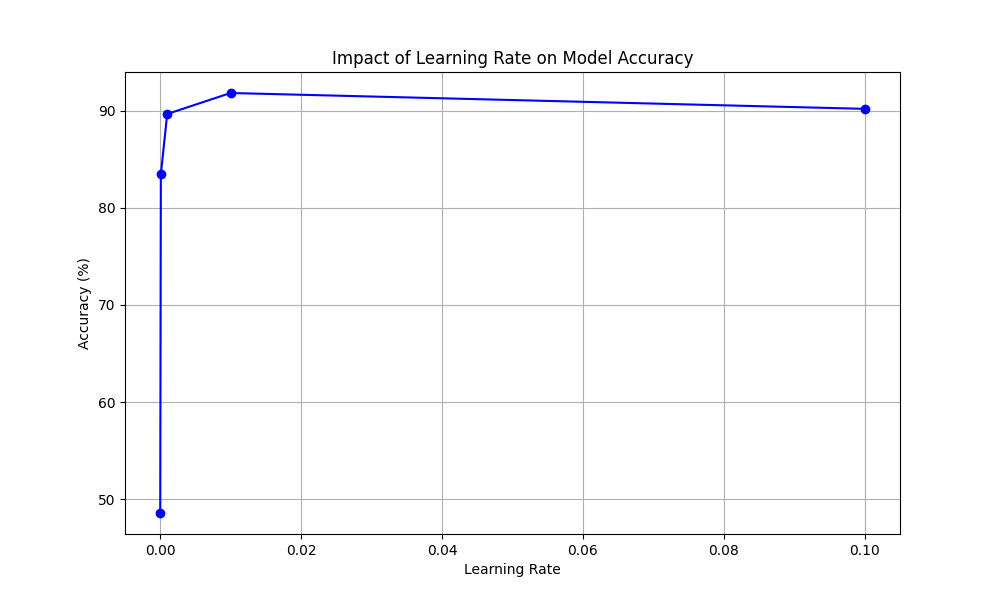
\includegraphics[width=\textwidth]{results/logreg/learning_rate_study.png}
    \caption{Logistic regression classification with learningrates in the range from $10^{-5}$ to $10^{-1}$. The biggest accuracy is 91\% achieved with learning rate 0.1.}
    \label{fig:LogRegLearningRate}
\end{figure}

\newpage
From Figure \ref{fig:LogRegEpochs} we can see that the accuracy converges after 10 epochs. A maximum accuracy of 92\% was achieved with 25 epochs, which gives a difference of 0.8\% from the lowest score from 5 epochs. 

\begin{figure}[H]
    \centering
    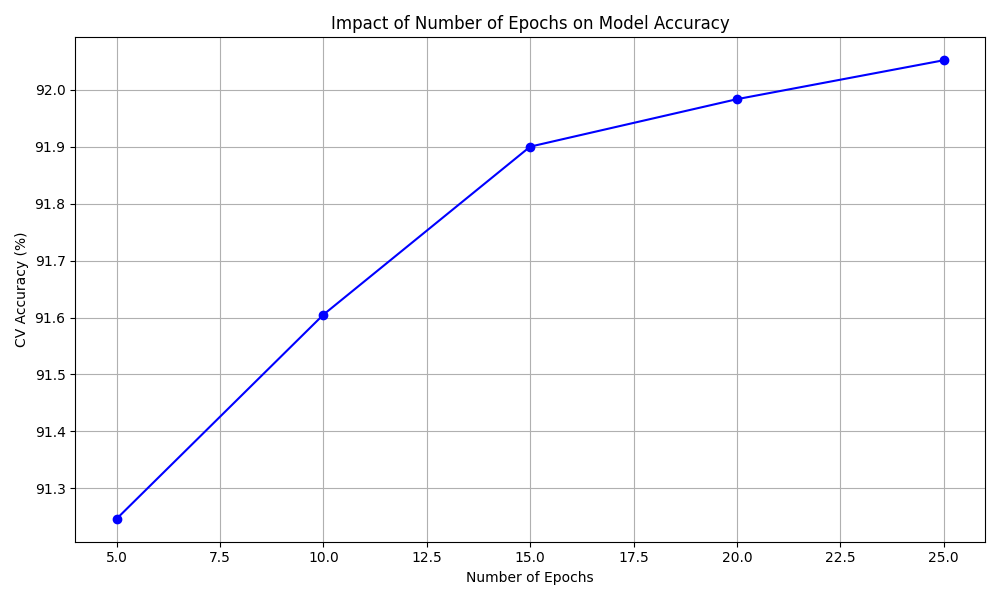
\includegraphics[width=\textwidth]{results/logreg/number_of_epochs_study.png}
    \caption{Logistic regression classification with epochs in the range from $5$ to $25$. The biggest accuracy achieved is 92\% with 25 epochs.}
    \label{fig:LogRegEpochs}
\end{figure}

\newpage
Referring to Figure \ref{fig:LogRegBatchsize}, we observe that, unlike the number of epochs, an increase in batch size results in lower accuracy. The highest accuracy of 91.8\% is achieved when a batch size 32 is used. In contrast a batch size of 256 gives the lowest accuracy of 90.8\%. It is important to note that the absolute decrease in accuracy is approximately 1\% for batch size and 0.8\% for epochs, which is relatively small. This suggests that these two variables are less critical for optimizing accuracy compared to the learning rate, which showed a 70\% difference between the lowest and highest values.

\begin{figure}[H]
    \centering
    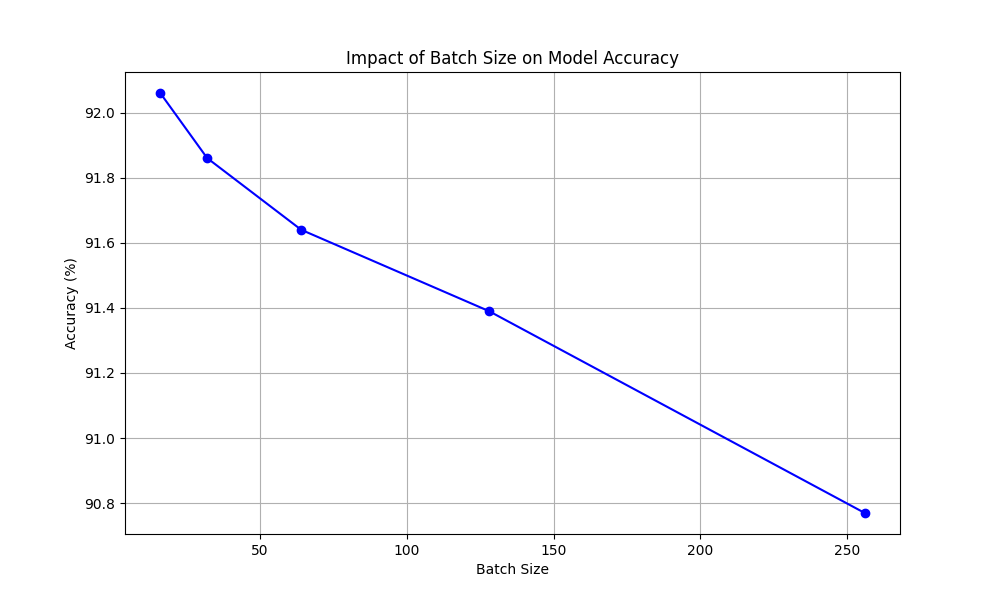
\includegraphics[width=\textwidth]{results/logreg/batch_size_study.png}
    \caption{Logistic regression classification with batchsize in the range from $16$ to $256$. The biggest accuracy achieved is 91.8\% when batch size is 32.}
    \label{fig:LogRegBatchsize}
\end{figure}

\newpage
\subsection{Results: Grid search on CNN}
\subsubsection{Number of Linear Layers and Convolutional Layers}
From Figure \ref{fig:cnn:layers}, we found that an additional convolutional layer and an additional linear layer increase the accuracy by 0.2\%, from 98.7\% to 98.9\% for our initial values. We decided to go on with this structure.
\begin{figure}[H]
    \centering
    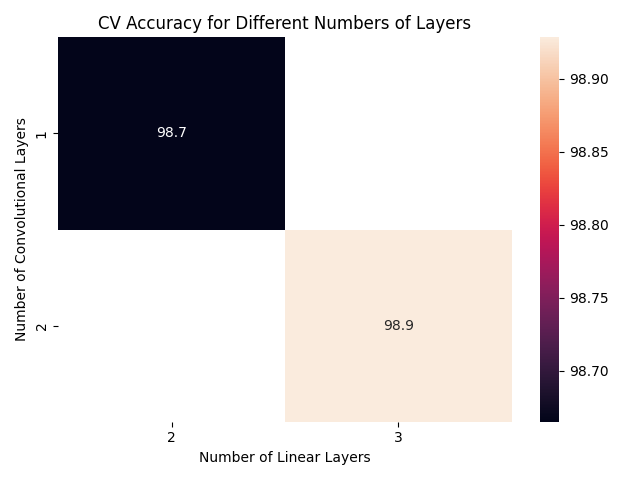
\includegraphics[width=\textwidth]{results/cnn_grid_search/heatmap_grid_search_layers.png}
    \caption{Results of a grid search comparing a convolutional neural network (CNN) with one convolutional layer followed by two linear layers, against a CNN with two convolutional layers followed by three linear layers.}
    \label{fig:cnn:layers}
\end{figure}

\newpage
\subsubsection{Kernel Size and Number of Filters}
Our results testing different kernel sizes and number of filters in the two convolutional layers are illustrated in Figure \ref{fig:cnn_kf}. We found that our initial structure of (32, 64) filters gave the best performance. Additionally, a kernel size of 5 performs better than 7 in all cases, and better than 3 for (32, 64) filters, so we continued with kernel size 5. The choice of a kernel size of 5 over 6 also benefits runtime too because a lower kernel size reduces computational load.
\begin{figure}[H]
    \centering
    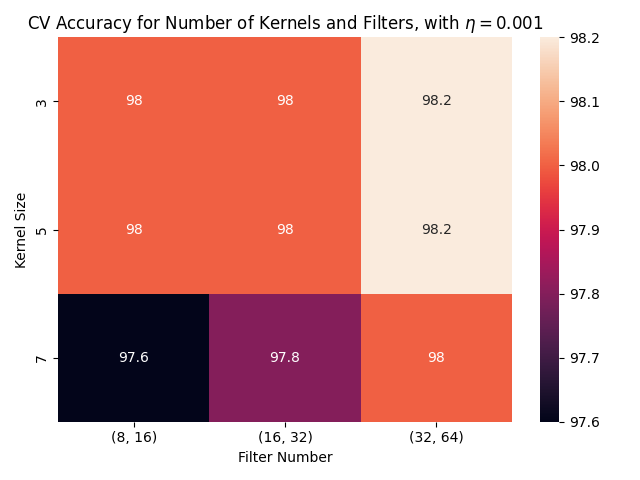
\includegraphics[width=\textwidth]{results/cnn_grid_search/heatmap_grid_search_kf.png}
    \caption{Results of a a grid search comparing differnent kernel sizes and number of filter in each of the two convolutional layers. Leraning rate is 0.001.}
    \label{fig:cnn_kf}
\end{figure}

\newpage
\subsubsection{Pooling and Padding}
Our grid search with pooling and convolutional layer padding is illustrated in Figure \ref{fig:cnn_pp}. It showed that adding padding had minimal impact on the cross-validated accuracy of the MNIST classifier. This makes sense as the MNIST dataset is digitally centered, with the edges of each image conveying minimal to no useful information about the digit pictured, which means the main utility of padding, better capturing information on the edge of the images, was not impactful. Additionally, we see that adding pooling layers with a kernel size of 2 after both convolutional layers did not result in a drop in performance.

\begin{figure}[H]
    \centering
    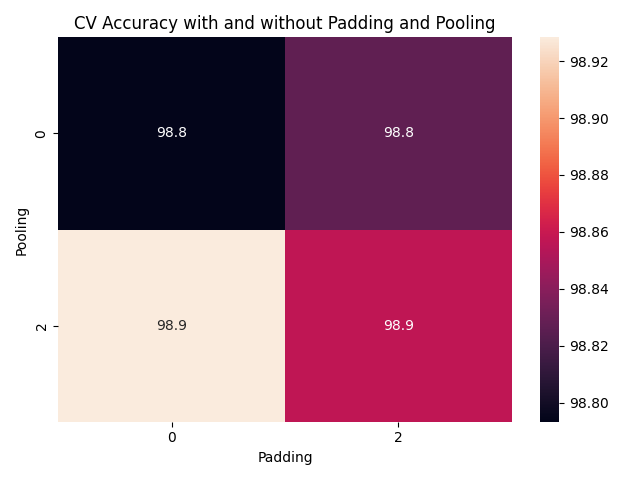
\includegraphics[width=\textwidth]{results/cnn_grid_search/heatmap_grid_search_pp.png}
    \caption{Heatmap reasults of Pooling and Padding grid search with two convolutional layers followed by three linear layers. The Y-axis represents pooling kernel size (0 means no pooling), with pooling layers placed after each convolutional layer, and the X-axis represents the convolutional layers' padding.}
    \label{fig:cnn_pp}
\end{figure}

In \ref{table:runtimes_pp} we see that the addition of padding increases runtimes drastically, while pooling conversely decreases it significantly. Taking into account the previously minimal performance increase and decrease of padding and pooling respectively, we identify no padding and pooling with a kernel size of 2 as the ideal configuration.

\begin{table}[H]
    \centering
    \caption{Runtime of cross-validation grid search of convolutional layer padding and subsequent pooling layers.}
    \label{table:runtimes_pp}
\begin{tabular}{|l|l|l|}
\hline
                    & \textbf{No Padding}      & \textbf{Padding: 2}      \\ \hline
\textbf{No Pooling} & 30 minutes 49.83 seconds & 57 minutes 28.26 seconds \\ \hline
\textbf{Pooling: 2} & 8 minutes 42.44 seconds  & 19 minutes 28.03 seconds \\ \hline
\end{tabular}
\end{table}

\newpage
\subsubsection{Dropout Rates and Activation Functions}
 Figure \ref{fig:cnn_pp} shows that the accuracy does not change much depending on dropout rate and activation functions. When running the code for 10 epochs, we got 98\% accuracy for all four combinations. We suspected our model structure and training time was too simple/short to get an effect of the dropout rate, due to our model not being prone to overfit. When increasing the number of epochs to 20, we got the same accuracy except for the case with LeakyRelu and Dropout rate 0.5, where the model achieved an accuracy of 98.2\%. This is the same performance as our previous implementation with 10 epochs and no dropout. In line with our selection criterion, we decided to go keep our implementation with 10 epochs and no dropout layer, with Relu as the activation function. 

\begin{figure}[H]
    \centering
    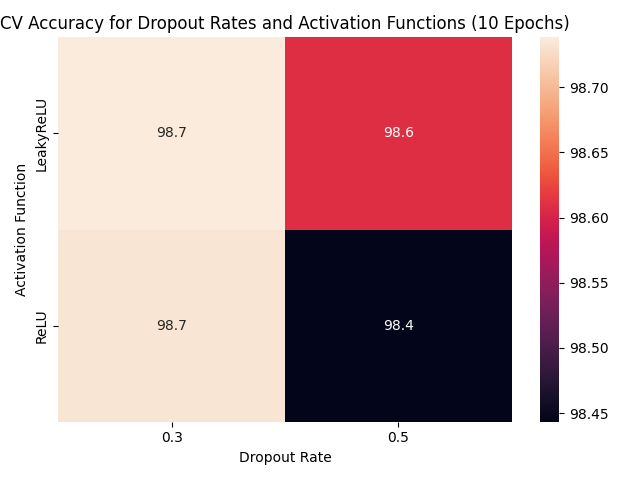
\includegraphics[width=\linewidth]{results/cnn_grid_search/heatmap_grid_search_da.png}
    \caption{Results of a a grid search experimenting with dropout rates and two different activation functions. We ran this result both with 10 and 20 epochs as we saw no change for 10 epochs, this plot is for 20 epochs. The results for 10 epochs can be found in the results folder of our code.}
    \label{fig:cnn_pp}
\end{figure}

We suspect that the small impact on accuracy from trying to avoid overregularization by using Leaky ReLU and dropout can be explained by the structure of the dataset. MNIST is a relatively simple dataset and as such may be less prone to overfitting. This could cause techniques intended to overcome this to be ineffective.

\subsection{Results: Final Assessment}

Figure \ref{fig:ClasswiseAccuracyLogReg} illustrates that the performance of Logistic Regression varies depending on the digit class. The difference in accuracy between the lowest-performing class, class 8, and the highest-performing classes, class 0 and class 1, is about 10\%. This variability is likely because logistic regression was originally designed for binary classification, and handling multiclass classification may be too complex for this model. The total accuracy on the test set without boostrap is 91.99\%, a small drop from the 92.72\% accuracy on the training set. For the boostrapped accuracy, Figure \ref{fig:appendix_ci} in Appendix \ref{sec:appendix} shows a 95\% confidence interval of [91.45, 92.54], reflecting that the performance of Logistic Regression varies between the digit classes, and thus between the different bootstrapped samples.
\begin{figure}[H]
    \centering
    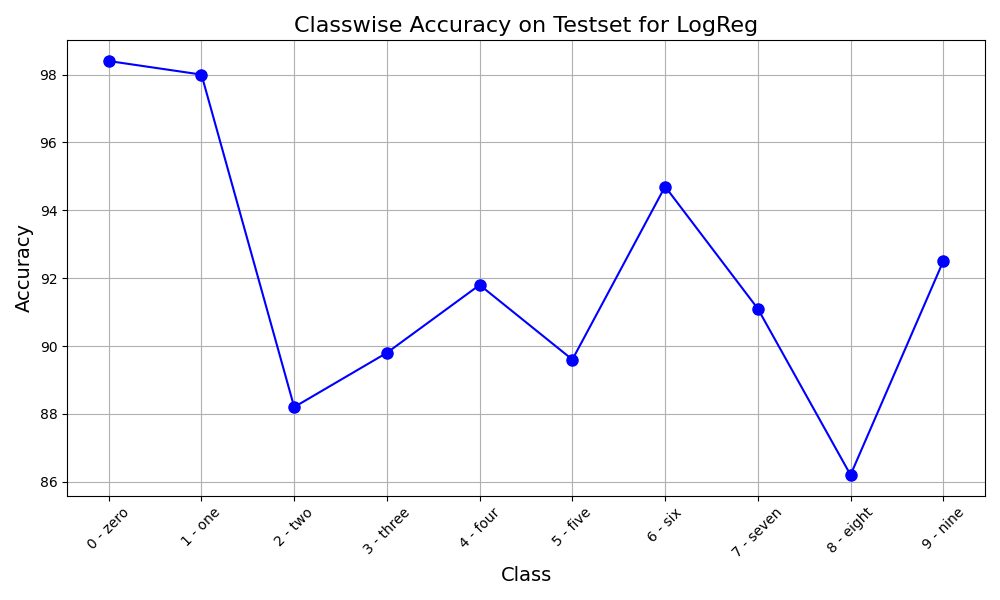
\includegraphics[width=\textwidth]{results/evaluation/LogReg_classwise_acc.png}
    \caption{Total accuracy of Logistic Regression on each class of number in the MNSIT dataset.}
    \label{fig:ClasswiseAccuracyLogReg}
\end{figure}

In contrast, Figure \ref{fig:ClasswiseAccuracyCNN} shows that the performance of our best CNN on each digit class is constistently high. The classwise performance drop is only about 2\%, ranging from the worst performance of 97.4\% on class 3 to the best performance of 99.6\% on class 1. One could suspect that the variation in performance is due to the model seeing more examples of the digit 1, as the first digit is more likely to be small than large in naturally occurring data sets, due to Benfords Law. It could also just be that the pattern of one and zero are easier to catch for the model structure. The stable performance compared to Logistic Regression confirms CNNs' ability to effectively handle classification of images. The accuracy on the whole test set is 98.86\%, a 1\% drop from the 99.66\% accuracy on the training set.
\begin{figure}[H]
    \centering
    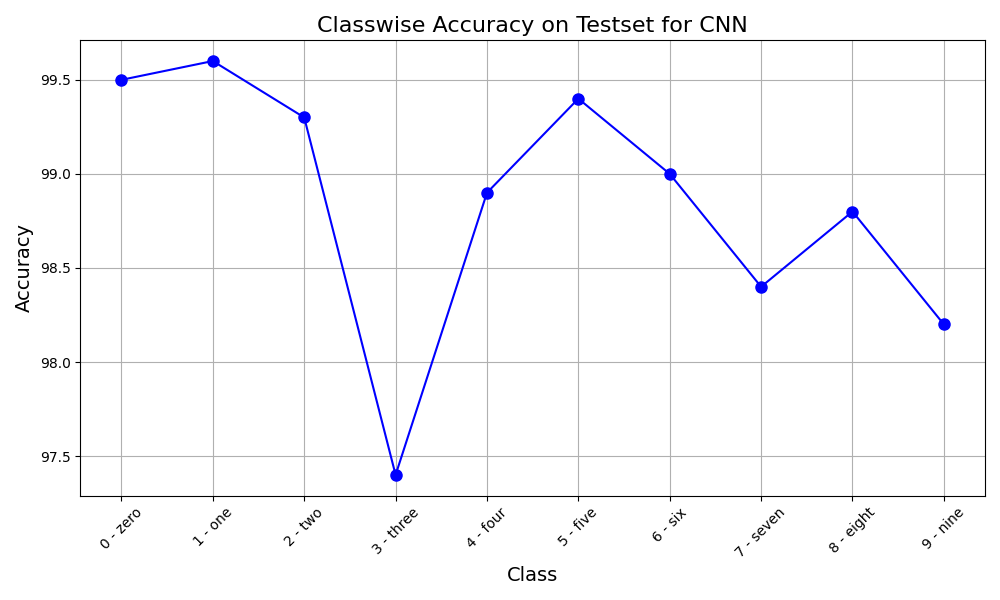
\includegraphics[width=\linewidth]{results/evaluation/CNN_classwise_acc.png}
    \caption{Our best CNNs performance on each class of number in the MNIST dataset.}
    \label{fig:ClasswiseAccuracyCNN}
\end{figure}

\newpage
Our bootstrapped accuracy in Figure \ref{fig:cnn_conf} shows that, for most of the bootstrapped test sets, the model performs close to the overall test set accuracy of 98.86\%, with a 95\% confidence interval of [98.66, 99.06]. This is significantly more narrow than the confidence interval of the Logistic Regression, reflecting that the CNN is more stable across the different digit classes. Our confidence interval indicates that even when the nature of our test set varies, the performance of our model does not change dramatically. This is a positive sign for deploying our model in a production setting with new data. 
Figure \ref{fig:cnn_conf} also shows that although the distribution of the bootstrapped accuracy has a clear mean and resembling a bell shape, it is somewhat spiky even though we run 1000 boostraps. This unexpected pattern is more likely due to the nature of our dataset rather than a problem with the model itself, as we observe some of the same effect with our baseline model (see Figure \ref{fig:appendix_ci} in Appendix \ref{sec:appendix}). Constructing a confidence interval by taking the percentiles of the boostrapped estimates assumes that the bootstrap distribution reasonably approximates the true sampling distribution. It could be that our data does not meet this assumption, possibly due to the MNIST data set being a preprocessed data set \cite{lecun1998gradient}.
\newline
\newline
\begin{figure}[H]
    \centering
    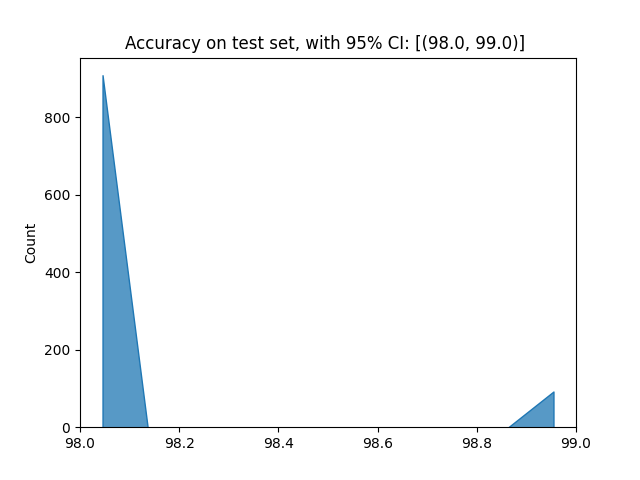
\includegraphics[width=\linewidth]{results/evaluation/cnn_confidence.png}
    \caption{The distribution of our best CNNs performance on the boostrapped MNIST dataset, with 1000 boostraps.}
    \label{fig:cnn_conf}
\end{figure}

\newpage
\subsection{Discussion}
As a benchmark, the best accuracy achieved on the MNIST dataset is 99.6\% \cite{simard2003mnist}. In contrast, we reached an accuracy of only 98\%, despite starting with good initial values. This demonstrates that extensive tuning is essential to develop highly accurate convolutional neural networks (CNNs). A key limitation in our approach was the high sensitivity of our results to the initial tuning values. In a neural network, all components are interrelated, which makes it challenging to isolate the effects of individual parameters.
\newline
\newline
Earlier in this course, we spent considerable time examining how factors such as learning rates, optimizers, and the number of epochs influence convergence and model performance. In this project, however, we focused on exploring hyperparameters specific to CNNs, such as filter numbers, kernel size, dropout, padding, and pooling. As a result, we devoted less attention to tuning basic parameters, which may have impacted our ability to achieve optimal performance.
\newline
\newline
Both the baseline logistic regression model and the CNN reached beyond 90\% accuracy, without an extensive tuning of the Logistic Regression model. This raises the question of whether using convolutional neural networks is worth the additional complexity, increased runtime, and reduced interpretability. However, in certain applications of a model trained on the MNIST dataset, such as reading bank account numbers from handwritten digits, even tiny errors can be very costly. Therefore, it is crucial to minimize these errors as much as possible \cite{raschka2022machine}. 
\newline
\newline
For tasks like digit recognition on the MNIST dataset, our results indicate that CNNs are worth the effort due to their superior ability to capture spatial hierarchies in image data. However, this is not to say that Logistic Regression is useless for this task. In certain cases, Logistic Regression may still be a viable option, especially for simpler applications or when computational resources are limited. 
